\documentclass{ximera}
%
%%% Begin Laad packages
%
\makeatletter
\@ifclassloaded{xourse}{%
    \typeout{Start loading preamble.tex (in a XOURSE)}%
    \def\isXourse{true}   % automatically defined; pre 112022 it had to be set 'manually' in a xourse
}{%
    \typeout{Start loading preamble.tex (NOT in a XOURSE)}%
}
\makeatother

\pgfplotsset{compat=1.16}

\usepackage{currfile}

% 201908/202301: PAS OP: babel en doclicense lijken problemen te veroorzaken in .jax bestand
% (wegens syntax error met toegevoegde \newcommands ...)
\pdfOnly{
    \usepackage[hyperxmp=false,type={CC},modifier={by-nc-sa},version={4.0}]{doclicense}
    \usepackage[dutch]{babel}
}


\usepackage[utf8]{inputenc}
\usepackage{morewrites}   % nav zomercursus (answer...?)
\usepackage{multirow}
\usepackage{multicol}
\usepackage{tikzsymbols}
\usepackage{tikz-3dplot}
\usepackage{ifthen}
%\usepackage{animate} BREAKS HTML STRUCTURE USED BY XIMERA
\usepackage{relsize}

\usepackage{eurosym}    % \euro  (€ werkt niet in xake ...?)
\usepackage{wrapfig}

\usepackage{cancel}

\usepackage{tabularx}
% Nuttig als ook interactieve beamer slides worden voorzien:
\providecommand{\p}{} % default nothing ; potentially usefull for slides: redefine as \pause
%providecommand{\p}{\pause}

\usepackage{caption} % captionof
%\usepackage{pdflscape}    % landscape environment

% Met "\newcommand\showtodonotes{}" kan je todonotes tonen (in pdf/online)
% 201908: online werkt het niet (goed)
\providecommand\showtodonotes{disable}
\providecommand\todo[1]{\typeout{TODO #1}}
%\usepackage[\showtodonotes]{todonotes}
%\usepackage{todonotes}

%
% Poging tot aanpassen layout
%
\usepackage{tcolorbox}
\tcbuselibrary{theorems}

%%% Einde laad packages

%%% Begin Ximera specifieke zaken

% \graphicspath{
% 	{../../}
% 	{../}
% 	{./}
%   	{../../pictures/}
%    	{../pictures/}
%    	{./pictures/}
% 	{./explog/}    % M05 in groeimodellen       
% }

%%% Einde Ximera specifieke zaken

%
% define softer blue/red/green, use KU Leuven base colors for blue (and dark orange for red ?)
%
% todo: rather redefine blue/red/green ...?
%\definecolor{xmblue}{rgb}{0.01, 0.31, 0.59}
%\definecolor{xmred}{rgb}{0.89, 0.02, 0.17}
\definecolor{xmdarkblue}{rgb}{0.122, 0.671, 0.835}   % KU Leuven Blauw
\definecolor{xmblue}{rgb}{0.114, 0.553, 0.69}        % KU Leuven Blauw
\definecolor{xmgreen}{rgb}{0.13, 0.55, 0.13}         % No KULeuven variant for green found ...

\definecolor{xmaccent}{rgb}{0.867, 0.541, 0.18}      % KU Leuven Accent (orange ...)
\definecolor{kuaccent}{rgb}{0.867, 0.541, 0.18}      % KU Leuven Accent (orange ...)

\colorlet{xmred}{xmaccent!50!black}                  % Darker version of KU Leuven Accent

\providecommand{\blue}[1]{{\color{blue}#1}}    
\providecommand{\red}[1]{{\color{red}#1}}

\renewcommand\CancelColor{\color{xmaccent!50!black}}

% werkt in math en text mode om MATH met oranje (of grijze...)  achtergond te tonen (ook \important{\text{blabla}} lijkt te werken)
%\newcommand{\important}[1]{\ensuremath{\colorbox{xmaccent!50!white}{$#1$}}}   % werkt niet in Mathjax
%\newcommand{\important}[1]{\ensuremath{\colorbox{lightgray}{$#1$}}}
%\newcommand{\important}[1]{\ensuremath{\colorbox{orange}{$#1$}}}   % TODO: kleur aanpassen voor mathjax; wordt overschreven infra!
\newcommand{\important}[1]{\ensuremath{\fcolorbox{black}{white}{$#1$}}}


% Uitzonderlijk kan met \pdfnl in de PDF een newline worden geforceerd, die online niet nodig/nuttig is omdat daar de regellengte hoe dan ook niet gekend is.
\ifdefined\HCode%
\providecommand{\pdfnl}{}%
\else%
\providecommand{\pdfnl}{%
  \\%
}%
\fi

% Uitzonderlijk kan met \handoutnl in de handout-PDF een newline worden geforceerd, die noch online noch in de PDF-met-antwoorden nuttig is.
\ifdefined\HCode
\providecommand{\handoutnl}{}
\else
\providecommand{\handoutnl}{%
\ifhandout%
  \nl%
\fi%
}
\fi



% \cellcolor IGNORED by tex4ht ?
% \begin{center} seems not to wordk
    % (missing margin-left: auto;   on tabular-inside-center ???)
%\newcommand{\importantcell}[1]{\ensuremath{\cellcolor{lightgray}#1}}  %  in tabular; usablility to be checked
\providecommand{\importantcell}[1]{\ensuremath{#1}}     % no mathjax2 support for colloring array cells

\pdfOnly{
  \renewcommand{\important}[1]{\ensuremath{\colorbox{kuaccent!50!white}{$#1$}}}
  \renewcommand{\importantcell}[1]{\ensuremath{\cellcolor{kuaccent!40!white}#1}}   
}

%%% Tikz styles


\pgfplotsset{compat=1.16}

\usetikzlibrary{trees,positioning,arrows,fit,shapes,math,calc,decorations.markings,through,intersections,patterns,matrix}

\usetikzlibrary{decorations.pathreplacing,backgrounds}    % 5/2023: from experimental


\usetikzlibrary{angles,quotes}

\usepgfplotslibrary{fillbetween} % bepaalde_integraal
\usepgfplotslibrary{polar}    % oa voor poolcoordinaten.tex

\pgfplotsset{ownstyle/.style={axis lines = center, axis equal image, xlabel = $x$, ylabel = $y$, enlargelimits}} 

\pgfplotsset{
	plot/.style={no marks,samples=50}
}

\newcommand{\xmPlotsColor}{
	\pgfplotsset{
		plot1/.style={darkgray,no marks,samples=100},
		plot2/.style={lightgray,no marks,samples=100},
		plotresult/.style={blue,no marks,samples=100},
		plotblue/.style={blue,no marks,samples=100},
		plotred/.style={red,no marks,samples=100},
		plotgreen/.style={green,no marks,samples=100},
		plotpurple/.style={purple,no marks,samples=100}
	}
}
\newcommand{\xmPlotsBlackWhite}{
	\pgfplotsset{
		plot1/.style={black,loosely dashed,no marks,samples=100},
		plot2/.style={black,loosely dotted,no marks,samples=100},
		plotresult/.style={black,no marks,samples=100},
		plotblue/.style={black,no marks,samples=100},
		plotred/.style={black,dotted,no marks,samples=100},
		plotgreen/.style={black,dashed,no marks,samples=100},
		plotpurple/.style={black,dashdotted,no marks,samples=100}
	}
}


\newcommand{\xmPlotsColorAndStyle}{
	\pgfplotsset{
		plot1/.style={darkgray,no marks,samples=100},
		plot2/.style={lightgray,no marks,samples=100},
		plotresult/.style={blue,no marks,samples=100},
		plotblue/.style={xmblue,no marks,samples=100},
		plotred/.style={xmred,dashed,thick,no marks,samples=100},
		plotgreen/.style={xmgreen,dotted,very thick,no marks,samples=100},
		plotpurple/.style={purple,no marks,samples=100}
	}
}


%\iftikzexport
\xmPlotsColorAndStyle
%\else
%\xmPlotsBlackWhite
%\fi
%%%


%
% Om venndiagrammen te arceren ...
%
\makeatletter
\pgfdeclarepatternformonly[\hatchdistance,\hatchthickness]{north east hatch}% name
{\pgfqpoint{-1pt}{-1pt}}% below left
{\pgfqpoint{\hatchdistance}{\hatchdistance}}% above right
{\pgfpoint{\hatchdistance-1pt}{\hatchdistance-1pt}}%
{
	\pgfsetcolor{\tikz@pattern@color}
	\pgfsetlinewidth{\hatchthickness}
	\pgfpathmoveto{\pgfqpoint{0pt}{0pt}}
	\pgfpathlineto{\pgfqpoint{\hatchdistance}{\hatchdistance}}
	\pgfusepath{stroke}
}
\pgfdeclarepatternformonly[\hatchdistance,\hatchthickness]{north west hatch}% name
{\pgfqpoint{-\hatchthickness}{-\hatchthickness}}% below left
{\pgfqpoint{\hatchdistance+\hatchthickness}{\hatchdistance+\hatchthickness}}% above right
{\pgfpoint{\hatchdistance}{\hatchdistance}}%
{
	\pgfsetcolor{\tikz@pattern@color}
	\pgfsetlinewidth{\hatchthickness}
	\pgfpathmoveto{\pgfqpoint{\hatchdistance+\hatchthickness}{-\hatchthickness}}
	\pgfpathlineto{\pgfqpoint{-\hatchthickness}{\hatchdistance+\hatchthickness}}
	\pgfusepath{stroke}
}
%\makeatother

\tikzset{
    hatch distance/.store in=\hatchdistance,
    hatch distance=10pt,
    hatch thickness/.store in=\hatchthickness,
   	hatch thickness=2pt
}

\colorlet{circle edge}{black}
\colorlet{circle area}{blue!20}


\tikzset{
    filled/.style={fill=green!30, draw=circle edge, thick},
    arceerl/.style={pattern=north east hatch, pattern color=blue!50, draw=circle edge},
    arceerr/.style={pattern=north west hatch, pattern color=yellow!50, draw=circle edge},
    outline/.style={draw=circle edge, thick}
}




%%% Updaten commando's
\def\hoofding #1#2#3{\maketitle}     % OBSOLETE ??

% we willen (bijna) altijd \geqslant ipv \geq ...!
\newcommand{\geqnoslant}{\geq}
\renewcommand{\geq}{\geqslant}
\newcommand{\leqnoslant}{\leq}
\renewcommand{\leq}{\leqslant}

% Todo: (201908) waarom komt er (soms) underlined voor emph ...?
\renewcommand{\emph}[1]{\textit{#1}}

% API commando's

\newcommand{\ds}{\displaystyle}
\newcommand{\ts}{\textstyle}  % tegenhanger van \ds   (Ximera zet PER  DEFAULT \ds!)

% uit Zomercursus-macro's: 
\newcommand{\bron}[1]{\begin{scriptsize} \emph{#1} \end{scriptsize}}     % deprecated ...?


%definities nieuwe commando's - afkortingen veel gebruikte symbolen
\newcommand{\R}{\ensuremath{\mathbb{R}}}
\newcommand{\Rnul}{\ensuremath{\mathbb{R}_0}}
\newcommand{\Reen}{\ensuremath{\mathbb{R}\setminus\{1\}}}
\newcommand{\Rnuleen}{\ensuremath{\mathbb{R}\setminus\{0,1\}}}
\newcommand{\Rplus}{\ensuremath{\mathbb{R}^+}}
\newcommand{\Rmin}{\ensuremath{\mathbb{R}^-}}
\newcommand{\Rnulplus}{\ensuremath{\mathbb{R}_0^+}}
\newcommand{\Rnulmin}{\ensuremath{\mathbb{R}_0^-}}
\newcommand{\Rnuleenplus}{\ensuremath{\mathbb{R}^+\setminus\{0,1\}}}
\newcommand{\N}{\ensuremath{\mathbb{N}}}
\newcommand{\Nnul}{\ensuremath{\mathbb{N}_0}}
\newcommand{\Z}{\ensuremath{\mathbb{Z}}}
\newcommand{\Znul}{\ensuremath{\mathbb{Z}_0}}
\newcommand{\Zplus}{\ensuremath{\mathbb{Z}^+}}
\newcommand{\Zmin}{\ensuremath{\mathbb{Z}^-}}
\newcommand{\Znulplus}{\ensuremath{\mathbb{Z}_0^+}}
\newcommand{\Znulmin}{\ensuremath{\mathbb{Z}_0^-}}
\newcommand{\C}{\ensuremath{\mathbb{C}}}
\newcommand{\Cnul}{\ensuremath{\mathbb{C}_0}}
\newcommand{\Cplus}{\ensuremath{\mathbb{C}^+}}
\newcommand{\Cmin}{\ensuremath{\mathbb{C}^-}}
\newcommand{\Cnulplus}{\ensuremath{\mathbb{C}_0^+}}
\newcommand{\Cnulmin}{\ensuremath{\mathbb{C}_0^-}}
\newcommand{\Q}{\ensuremath{\mathbb{Q}}}
\newcommand{\Qnul}{\ensuremath{\mathbb{Q}_0}}
\newcommand{\Qplus}{\ensuremath{\mathbb{Q}^+}}
\newcommand{\Qmin}{\ensuremath{\mathbb{Q}^-}}
\newcommand{\Qnulplus}{\ensuremath{\mathbb{Q}_0^+}}
\newcommand{\Qnulmin}{\ensuremath{\mathbb{Q}_0^-}}

\newcommand{\perdef}{\overset{\mathrm{def}}{=}}
\newcommand{\pernot}{\overset{\mathrm{notatie}}{=}}
\newcommand\perinderdaad{\overset{!}{=}}     % voorlopig gebruikt in limietenrekenregels
\newcommand\perhaps{\overset{?}{=}}          % voorlopig gebruikt in limietenrekenregels

\newcommand{\degree}{^\circ}


\DeclareMathOperator{\dom}{dom}     % domein
\DeclareMathOperator{\codom}{codom} % codomein
\DeclareMathOperator{\bld}{bld}     % beeld
\DeclareMathOperator{\graf}{graf}   % grafiek
\DeclareMathOperator{\rico}{rico}   % richtingcoëfficient
\DeclareMathOperator{\co}{co}       % coordinaat
\DeclareMathOperator{\gr}{gr}       % graad

\newcommand{\func}[5]{\ensuremath{#1: #2 \rightarrow #3: #4 \mapsto #5}} % Easy to write a function


% Operators
\DeclareMathOperator{\bgsin}{bgsin}
\DeclareMathOperator{\bgcos}{bgcos}
\DeclareMathOperator{\bgtan}{bgtan}
\DeclareMathOperator{\bgcot}{bgcot}
\DeclareMathOperator{\bgsinh}{bgsinh}
\DeclareMathOperator{\bgcosh}{bgcosh}
\DeclareMathOperator{\bgtanh}{bgtanh}
\DeclareMathOperator{\bgcoth}{bgcoth}

% Oude \Bgsin etc deprecated: gebruik \bgsin, en herdefinieer dat als je Bgsin wil!
%\DeclareMathOperator{\cosec}{cosec}    % not used? gebruik \csc en herdefinieer

% operatoren voor differentialen: to be verified; 1/2020: inconsequent gebruik bij afgeleiden/integralen
\renewcommand{\d}{\mathrm{d}}
\newcommand{\dx}{\d x}
\newcommand{\dd}[1]{\frac{\mathrm{d}}{\mathrm{d}#1}}
\newcommand{\ddx}{\dd{x}}

% om in voorbeelden/oefeningen de notatie voor afgeleiden te kunnen kiezen
% Usage: \afg{(2\sin(x))}  (en wordt d/dx, of accent, of D )
% \afg kan evt al gedefinieerd zijn in xmPreamble, of overschreven worden  
\providecommand{\afg}[1]{\frac{\mathrm{d}}{\mathrm{d}x} \left(#1\right) }   % include in relevant exercises ...
% \providecommand{\afg}[1]{\left{#1\right}'}   
%\renewcommand{\afg}[1]{D\left{#1\right}}

%
% \xmxxx commands: Extra KU Leuven functionaliteit van, boven of naast Ximera
%   ( Conventie 8/2019: xm+nederlandse omschrijving, maar is niet consequent gevolgd, en misschien ook niet erg handig !)
%
% (Met een minimale ximera.cls en preamble.tex zou een bruikbare .pdf moeten kunnen worden gemaakt van eender welke ximera)
%
% Usage: \xmtitle[Mijn korte abstract]{Mijn titel}{Mijn abstract}
% Eerste command na \begin{document}:
%  -> definieert de \title
%  -> definieert de abstract
%  -> doet \maketitle ( dus: print de hoofding als 'chapter' of 'sectie')
% Optionele parameter geeft eenn kort abstract (die met de globale setting \xmshortabstract{} al dan niet kan worden geprint.
% De optionele korte abstract kan worden gebruikt voor pseudo-grappige abtsarts, dus dus globaal al dan niet kunnen worden gebuikt...
% Globale settings:
%  de (optionele) 'korte abstract' wordt enkele getoond als \xmshortabstract is gezet
\providecommand\xmshortabstract{} % default: print (only!) short abstract if present
\providecommand\theabstract{} % otherwise complaint Undefined control sequence.  <recently read> \theabstract  ????
\newcommand{\xmtitle}[3][]{
	\title{#2}
	% \begin{abstract}
	% 			\ifdefined\xmshortabstract
	% 			\ifstrempty{#1}{%
	% 						#3
	% 			}{%
	% 						#1
	% 			}%
	% 			\else
	% 			#3
	% 			\fi
	% \end{abstract}
	\maketitle
}

% 
% Kleine grapjes: moeten zonder verder gevolg kunnen worden verwijderd
%
%\newcommand{\xmopje}[1]{{\small#1{\reversemarginpar\marginpar{\Smiley}}}}   % probleem in floats!!
\newtoggle{showxmopje}
\toggletrue{showxmopje}

\newcommand{\xmopje}[1]{%
   \iftoggle{showxmopje}{#1}{}%
}


% -> geef een abstracte-formule-met-rechts-een-concreet-voorbeeld
% VB:  \formulevb{a^2+b^2=c^2}{3^2+4^2=5^2}
%
\ifdefined\HCode
\NewEnviron{xmdiv}[1]{\HCode{\Hnewline<div class="#1">\Hnewline}\BODY{\HCode{\Hnewline</div>\Hnewline}}}
\else
\NewEnviron{xmdiv}[1]{\BODY}
\fi

\providecommand{\formulevb}[2]{
	{\centering

    \begin{xmdiv}{xmformulevb}    % zie css voor online layout !!!
	\begin{tabular}{lcl}
		\important{#1}
		&  &
		 {$#2$}
		\end{tabular}
	\end{xmdiv}
	}
}

\ifdefined\HCode
\providecommand{\xmcolorbox}[2]{
	\HCode{\Hnewline<div class="xmcolorbox">\Hnewline}#2\HCode{\Hnewline</div>\Hnewline}
}
\else
\providecommand{\xmcolorbox}[2]{
  \cellcolor{#1}#2
}
\fi


\ifdefined\HCode
\providecommand{\xmopmerking}[1]{
 \HCode{\Hnewline<div class="xmopmerking">\Hnewline}#1\HCode{\Hnewline</div>\Hnewline}
}
\else
\providecommand{\xmopmerking}[1]{
	{\footnotesize #1}
}
\fi
% \providecommand{\voorbeeld}[1]{
% 	\colorbox{blue!10}{$#1$}
% }



% Hernoem Proof naar Bewijs, nodig voor HTML versie
\renewcommand*{\proofname}{Bewijs}

% Om opgave van oefening (wordt niet geprint bij oplossingenblad)
% (to be tested test)
\NewEnviron{statement}{\BODY}

% Environment 'oplossing' en 'uitkomst'
% voor resp. volledige 'uitwerking' dan wel 'enkel eindresultaat'
% geimplementeerd via feedback, omdat er in de ximera-server adhoc feedback-code is toegevoegd
%% Niet tonen indien handout
%% Te gebruiken om volledige oplossingen/uitwerkingen van oefeningen te tonen
%% \begin{oplossing}        De optelling is commutatief \end{oplossing}  : verschijnt online enkel 'op vraag'
%% \begin{oplossing}[toon]  De optelling is commutatief \end{oplossing}  : verschijnt steeds onmiddellijk online (bv te gebruiken bij voorbeelden) 

\ifhandout%
    \NewEnviron{oplossing}[1][onzichtbaar]%
    {%
    \ifthenelse{\equal{\detokenize{#1}}{\detokenize{toon}}}
    {
    \def\PH@Command{#1}% Use PH@Command to hold the content and be a target for "\expandafter" to expand once.

    \begin{trivlist}% Begin the trivlist to use formating of the "Feedback" label.
    \item[\hskip \labelsep\small\slshape\bfseries Oplossing% Format the "Feedback" label. Don't forget the space.
    %(\texttt{\detokenize\expandafter{\PH@Command}}):% Format (and detokenize) the condition for feedback to trigger
    \hspace{2ex}]\small%\slshape% Insert some space before the actual feedback given.
    \BODY
    \end{trivlist}
    }
    {  % \begin{feedback}[solution]   \BODY     \end{feedback}  }
    }
    }    
\else
% ONLY for HTML; xmoplossing is styled with css, and is not, and need not be a LaTeX environment
% THUS: it does NOT use feedback anymore ...
%    \NewEnviron{oplossing}{\begin{expandable}{xmoplossing}{\nlen{Toon uitwerking}{Show solution}}{\BODY}\end{expandable}}
    \newenvironment{oplossing}[1][onzichtbaar]
   {%
       \begin{expandable}{xmoplossing}{}
   }
   {%
   	   \end{expandable}
   } 
%     \newenvironment{oplossing}[1][onzichtbaar]
%    {%
%        \begin{feedback}[solution]   	
%    }
%    {%
%    	   \end{feedback}
%    } 
\fi

\ifhandout%
    \NewEnviron{uitkomst}[1][onzichtbaar]%
    {%
    \ifthenelse{\equal{\detokenize{#1}}{\detokenize{toon}}}
    {
    \def\PH@Command{#1}% Use PH@Command to hold the content and be a target for "\expandafter" to expand once.

    \begin{trivlist}% Begin the trivlist to use formating of the "Feedback" label.
    \item[\hskip \labelsep\small\slshape\bfseries Uitkomst:% Format the "Feedback" label. Don't forget the space.
    %(\texttt{\detokenize\expandafter{\PH@Command}}):% Format (and detokenize) the condition for feedback to trigger
    \hspace{2ex}]\small%\slshape% Insert some space before the actual feedback given.
    \BODY
    \end{trivlist}
    }
    {  % \begin{feedback}[solution]   \BODY     \end{feedback}  }
    }
    }    
\else
\ifdefined\HCode
   \newenvironment{uitkomst}[1][onzichtbaar]
    {%
        \begin{expandable}{xmuitkomst}{}%
    }
    {%
    	\end{expandable}%
    } 
\else
  % Do NOT print 'uitkomst' in non-handout
  %  (presumably, there is also an 'oplossing' ??)
  \newenvironment{uitkomst}[1][onzichtbaar]{}{}
\fi
\fi

%
% Uitweidingen zijn extra's die niet redelijkerwijze tot de leerstof behoren
% Uitbreidingen zijn extra's die wel redelijkerwijze tot de leerstof van bv meer geavanceerde versies kunnen behoren (B-programma/Wiskundestudenten/...?)
% Nog niet voorzien: design voor verschillende versies (A/B programma, BIO, voorkennis/ ...)
% Voor 'uitweidingen' is er een environment die online per default is ingeklapt, en in pdf al dan niet kan worden geincluded  (via \xmnouitweiding) 
%
% in een xourse, per default GEEN uitweidingen, tenzij \xmuitweiding expliciet ergens is gezet ...
\ifdefined\isXourse
   \ifdefined\xmuitweiding
   \else
       \def\xmnouitweiding{true}
   \fi
\fi

\ifdefined\xmnouitweiding
\newcounter{xmuitweiding}  % anders error undefined ...  
\excludecomment{xmuitweiding}
\else
\newtheoremstyle{dotless}{}{}{}{}{}{}{ }{}
\theoremstyle{dotless}
\newtheorem*{xmuitweidingnofrills}{}   % nofrills = no accordion; gebruikt dus de dotless theoremstyle!

\newcounter{xmuitweiding}
\newenvironment{xmuitweiding}[1][ ]%
{% 
	\refstepcounter{xmuitweiding}%
    \begin{expandable}{xmuitweiding}{Uitweiding \arabic{xmuitweiding}: #1}%
	\begin{xmuitweidingnofrills}%
}
{%
    \end{xmuitweidingnofrills}%
    \end{expandable}%
}   
% \newenvironment{xmuitweiding}[1][ ]%
% {% 
% 	\refstepcounter{xmuitweiding}
% 	\begin{accordion}\begin{accordion-item}[Uitweiding \arabic{xmuitweiding}: #1]%
% 			\begin{xmuitweidingnofrills}%
% 			}
% 			{\end{xmuitweidingnofrills}\end{accordion-item}\end{accordion}}   
\fi


\newenvironment{xmexpandable}[1][]{
	\begin{accordion}\begin{accordion-item}[#1]%
		}{\end{accordion-item}\end{accordion}}


% Command that gives a selection box online, but just prints the right answer in pdf
\newcommand{\xmonlineChoice}[1]{\pdfOnly{\wordchoicegiventrue}\wordChoice{#1}\pdfOnly{\wordchoicegivenfalse}}   % deprecated, gebruik onlineChoice ...
\newcommand{\onlineChoice}[1]{\pdfOnly{\wordchoicegiventrue}\wordChoice{#1}\pdfOnly{\wordchoicegivenfalse}}

\newcommand{\TJa}{\nlentext{ Ja }{ Yes }}
\newcommand{\TNee}{\nlentext{ Nee }{ No }}
\newcommand{\TJuist}{\nlentext{ Juist }{ True }}
\newcommand{\TFout}{\nlentext{ Fout }{ False }}

\newcommand{\choiceTrue}{{\wordChoice{\choice[correct]{\TJuist}\choice{\TFout}}}}
\newcommand{\choiceFalse}{{\wordChoice{\choice{\TJuist}\choice[correct]{\TFout}}}}

\newcommand{\choiceYes}{{\wordChoice{\choice[correct]{\TJa}\choice{\TNee}}}}
\newcommand{\choiceNo}{{\wordChoice{\choice{\TJa}\choice[correct]{\TNee}}}}

\newcommand{\choiceEen}{{\wordChoice{\choice[correct]{een }\choice{geen }}}}
\newcommand{\choiceGeen}{{\wordChoice{\choice{een }\choice[correct]{geen }}}}

% Optional nicer formatting for wordChoice in PDF

\let\inlinechoiceorig\inlinechoice

%\makeatletter
%\providecommand{\choiceminimumverticalsize}{\vphantom{$\frac{\sqrt{2}}{2}$}}   % minimum height of boxes (cfr infra)
\providecommand{\choiceminimumverticalsize}{\vphantom{$\tfrac{2}{2}$}}   % minimum height of boxes (cfr infra)

\newcommand{\inlinechoicesquares}[2][]{%
		\setkeys{choice}{#1}%
		\ifthenelse{\boolean{\choice@correct}}%
		{%
            \ifhandout%
               \fbox{\choiceminimumverticalsize #2}\allowbreak\ignorespaces%
            \else%
               \fcolorbox{blue}{blue!20}{\choiceminimumverticalsize #2\checkmark}\allowbreak\ignorespaces\setkeys{choice}{correct=false}\ignorespaces%
            \fi%
		}%
		{% else
			\fbox{\choiceminimumverticalsize #2}\allowbreak\ignorespaces%  HACK: wat kleiner, zodat fits on line ... 	
		}%
}

\newcommand{\inlinechoicesquareX}[2][]{%
		\setkeys{choice}{#1}%
		\ifthenelse{\boolean{\choice@correct}}%
		{%
            \ifhandout%
               \fbox{\choiceminimumverticalsize #2}\allowbreak\ignorespaces\setkeys{choice}{correct=false}\ignorespaces%
            \else%
               \fcolorbox{blue}{blue!20}{\choiceminimumverticalsize #2\checkmark}\allowbreak\ignorespaces\setkeys{choice}{correct=false}\ignorespaces%
            \fi%
		}%
		{% else
        \ifhandout%
			\fbox{\choiceminimumverticalsize #2}\allowbreak\ignorespaces%  HACK: wat kleiner, zodat fits on line ... 	
        \fi
		}%
}


\newcommand{\inlinechoicepuntjes}[2][]{%
		\setkeys{choice}{#1}%
		\ifthenelse{\boolean{\choice@correct}}%
		{%
            \ifhandout%
               \dots\ldots\ignorespaces\setkeys{choice}{correct=false}\ignorespaces
            \else%
               \fcolorbox{blue}{blue!20}{\choiceminimumverticalsize #2}\allowbreak\ignorespaces\setkeys{choice}{correct=false}\ignorespaces%
            \fi%
		}%
		{% else
			%\fbox{\choiceminimumverticalsize #2}\allowbreak\ignorespaces%  HACK: wat kleiner, zodat fits on line ... 	
		}%
}

% print niets, maar definieer globale variable \myanswer
%  (gebruikt om oplossingsbladen te printen) 
\newcommand{\inlinechoicedefanswer}[2][]{%
		\setkeys{choice}{#1}%
		\ifthenelse{\boolean{\choice@correct}}%
		{%
               \gdef\myanswer{#2}\setkeys{choice}{correct=false}

		}%
		{% else
			%\fbox{\choiceminimumverticalsize #2}\allowbreak\ignorespaces%  HACK: wat kleiner, zodat fits on line ... 	
		}%
}



%\makeatother

\newcommand{\setchoicedefanswer}{
\ifdefined\HCode
\else
%    \renewenvironment{multipleChoice@}[1][]{}{} % remove trailing ')'
    \let\inlinechoice\inlinechoicedefanswer
\fi
}

\newcommand{\setchoicepuntjes}{
\ifdefined\HCode
\else
    \renewenvironment{multipleChoice@}[1][]{}{} % remove trailing ')'
    \let\inlinechoice\inlinechoicepuntjes
\fi
}
\newcommand{\setchoicesquares}{
\ifdefined\HCode
\else
    \renewenvironment{multipleChoice@}[1][]{}{} % remove trailing ')'
    \let\inlinechoice\inlinechoicesquares
\fi
}
%
\newcommand{\setchoicesquareX}{
\ifdefined\HCode
\else
    \renewenvironment{multipleChoice@}[1][]{}{} % remove trailing ')'
    \let\inlinechoice\inlinechoicesquareX
\fi
}
%
\newcommand{\setchoicelist}{
\ifdefined\HCode
\else
    \renewenvironment{multipleChoice@}[1][]{}{)}% re-add trailing ')'
    \let\inlinechoice\inlinechoiceorig
\fi
}

\setchoicesquareX  % by default list-of-squares with onlineChoice in PDF

% Omdat multicols niet werkt in html: enkel in pdf  (in html zijn langere pagina's misschien ook minder storend)
\newenvironment{xmmulticols}[1][2]{
 \pdfOnly{\begin{multicols}{#1}}%
}{ \pdfOnly{\end{multicols}}}

%
% Te gebruiken in plaats van \section\subsection
%  (in een printstyle kan dan het level worden aangepast
%    naargelang \chapter vs \section style )
% 3/2021: DO NOT USE \xmsubsection !
\newcommand\xmsection\subsection
\newcommand\xmsubsection\subsubsection

% Aanpassen printversie
%  (hier gedefinieerd, zodat ze in xourse kunnen worden gezet/overschreven)
\providebool{parttoc}
\providebool{printpartfrontpage}
\providebool{printactivitytitle}
\providebool{printactivityqrcode}
\providebool{printactivityurl}
\providebool{printcontinuouspagenumbers}


\providebool{printquickquestion}
\printquickquestiontrue

% The following three commands are hardcoded in xake, you can't create other commands like these, without adding them to xake as well
%  ( gebruikt in xourses om juiste soort titelpagina te krijgen voor verschillende ximera's )
\newcommand{\activitychapter}[1]{
	\typeout{ACTIVITYCHAPTER #1}   % logging
	\chapterstyle
	\activity{#1}
}
\newcommand{\activitysection}[1]{
	\typeout{ACTIVITYSECTION #1}   % logging
	\sectionstyle
	\activity{#1}
}
% Partices worden als activity getoond om de grote blokken te krijgen online
\newcommand{\practicesection}[1]{
	\typeout{PRACTICESECTION #1}   % logging
	\sectionstyle
	\activity{#1}
}


% Commando om de printstyle toe te voegen in ximera's. Zorgt ervoor dat er geen problemen zijn als je de xourses compileert
% hack om onhandige relative paden in TeX te omzeilen
% should work both in xourse and ximera (pre-112022 only in ximera; thus obsoletes adhoc setup in xourses)
% loads global.sty if present (cfr global.css for online settings!)
% use global.sty to overwrite settings in printstyle.sty ...
\newcommand{\addPrintStyle}[1]{
\iftikzexport\else   % only in PDF
  \makeatletter
  \ifx\@onlypreamble\@notprerr\else   % ONLY if in tex-preamble   (and e.g. not when included from xourse)
    \typeout{Loading printstyle}   % logging
    \usepackage{#1/printstyle} % mag enkel geinclude worden als je die apart compileert
    \IfFileExists{#1/global.sty}{
        \typeout{Loading printstyle-folder #1/global.sty}   % logging
        \usepackage{#1/global}
        }{
        \typeout{Info: No extra #1/global.sty}   % logging
    }   % load global.sty if present
    \IfFileExists{global.sty}{
        \typeout{Loading local-folder global.sty (or TEXINPUTPATH..)}   % logging
        \usepackage{global}
    }{
        \typeout{Info: No folder/global.sty}   % logging
    }   % load global.sty if present
    \IfFileExists{\currfilebase.sty}
    {
        \typeout{Loading \currfilebase.sty}
        \input{\currfilebase.sty}
    }{
        \typeout{Info: No local \currfilebase.sty}
    }
    \fi
  \makeatother
\fi
}

%
%  
% references: Ximera heeft adhoc logica	 om online labels te doen werken over verschillende files heen
% met \hyperref kan de getoonde tekst toch worden opgegeven, in plaats van af te hangen van de label-text
\ifdefined\HCode
% Link to standard \labels, but give your own description
% Usage:  Volg \hyperref[my_very_verbose_label]{deze link} voor wat tijdverlies
%   (01/2020: Ximera-server aangepast om bij class reference-keeptext de link-text NIET te vervangen door de label-text !!!) 
\renewcommand{\hyperref}[2][]{\HCode{<a class="reference reference-keeptext" href="\##1">}#2\HCode{</a>}}
%
%  Link to specific targets  (not tested ?)
\renewcommand{\hypertarget}[1]{\HCode{<a class="ximera-label" id="#1"></a>}}
\renewcommand{\hyperlink}[2]{\HCode{<a class="reference reference-keeptext" href="\##1">}#2\HCode{</a>}}
\fi


\renewcommand{\figurename}{Figuur}
\renewcommand{\tablename}{Tabel}

%
% Gedoe om verschillende versies van xourse/ximera te maken afhankelijk van settings
%
% default: versie met antwoorden
% handout: versie voor de studenten, zonder antwoorden/oplossingen
% full: met alles erop en eraan, dus geschikt voor auteurs en/of lesgevers  (bevat in de pdf ook de 'online-only' stukken!)
%
%
% verder kunnen ook opties/variabele worden gezet voor hints/auteurs/uitweidingen/ etc
%
% 'Full' versie
\newtoggle{showonline}
\ifdefined\HCode   % zet default showOnline
    \toggletrue{showonline} 
\else
    \togglefalse{showonline}
\fi

% Full versie   % deprecated: see infra
\newcommand{\printFull}{
    \hintstrue
    \handoutfalse
    \toggletrue{showonline} 
}

\ifdefined\shouldPrintFull   % deprecated: see infra
    \printFull
\fi

%% \onlineOnly kan jammer genoeg niet, omdat het al betsaat als neveneffect van \begin{onlineOnly} ...
\newcommand{\onlyOnline}[1]{\ifdefined\HCode#1\fi}

% Overschrijf onlineOnly  (zoals gedefinieerd in ximera.cls)
\ifhandout   % in handout: gebruik de oorspronkelijke ximera.cls implementatie  (is dit wel nodig/nuttig?)
\else
    \iftoggle{showonline}{%
        \ifdefined\HCode
          \RenewEnviron{onlineOnly}{\bgroup\BODY\egroup}   % showOnline, en we zijn  online, dus toon de tekst
        \else
          \RenewEnviron{onlineOnly}{\bgroup\color{red!50!black}\BODY\egroup}   % showOnline, maar we zijn toch niet online: kleur de tekst rood 
        \fi
    }{%
      \RenewEnviron{onlineOnly}{\setbox0\vbox\bgroup\BODY\egroup}% geen showOnline
    }
\fi

% hack om na hoofding van definition/proposition/... als dan niet op een nieuwe lijn te starten
% soms is dat goed en mooi, en soms niet; en in HTML is het nu (2/2020) anders dan in pdf
% vandaar suggestie om 
%     \begin{definition}[Nieuw concept] \nl
% te gebruiken als je zeker een newline wil na de hoofdig en titel
% (in het bijzonder itemize zonder \nl is 'lelijk' ...)
\ifdefined\HCode
\newcommand{\nl}{\Hnewline}
\else
\newcommand{\nl}{\ \par} % newline (achter heading van definition etc.)
\fi


% \nl enkel in handoutmode (ihb voor \wordChoice, die dan typisch veeeel langer wordt)
\ifdefined\HCode
\providecommand{\handoutnl}{}
\else
\providecommand{\handoutnl}{%
\ifhandout%
  \nl%
\fi%
}
\fi

% Could potentially replace \pdfOnline/\begin{onlineOnly} : 
% Usage= \ifonline{Hallo surfer}{Hallo PDFlezer}
\providecommand{\ifonline}[2]%
{
\begin{onlineOnly}#1\end{onlineOnly}%
\pdfOnly{#2}
}%


%
% Maak optionele 'basic' en 'extended' versies van een activity
%  met environment basicOnly, basicSkip en extendedOnly
%
%  (
%   Dit werkt ENKEL in de PDF; de online versies tonen (minstens voorklopig) steeds 
%   het default geval met printbasicversion en printextendversion beide FALSE
%  )
%
\providebool{printbasicversion}
\providebool{printextendedversion}   % not properly implemented
\providebool{printfullversion}       % presumably print everything (debug/auteur)
%
% only set these in xourses, and BEFORE loading this preamble
%
%\newif\ifshowbasic     \showbasictrue        % use this line in xourse to show 'basic' sections
%\newif\ifshowextended  \showextendedtrue     % use this line in xourse to show 'extended' sections
%
%
%\ifbool{showbasic}
%      { \NewEnviron{basicOnly}{\BODY} }    % if yes: just print contents
%      { \NewEnviron{basicOnly}{}      }    % if no:  completely ignore contents
%
%\ifbool{showbasic}
%      { \NewEnviron{basicSkip}{}      }
%      { \NewEnviron{basicSkip}{\BODY} }
%

\ifbool{printextendedversion}
      { \NewEnviron{extendedOnly}{\BODY} }
      { \NewEnviron{extendedOnly}{}      }
      


\ifdefined\HCode    % in html: always print
      \newenvironment*{basicOnly}{}{}    % if yes: just print contents
      \newenvironment*{basicSkip}{}{}    % if yes: just print contents
\else

\ifbool{printbasicversion}
      {\newenvironment*{basicOnly}{}{}}    % if yes: just print contents
      {\NewEnviron{basicOnly}{}      }    % if no:  completely ignore contents

\ifbool{printbasicversion}
      {\NewEnviron{basicSkip}{}      }
      {\newenvironment*{basicSkip}{}{}}

\fi

\usepackage{float}
\usepackage[rightbars,color]{changebar}

% Full versie
\ifbool{printfullversion}{
    \hintstrue
    \handoutfalse
    \toggletrue{showonline}
    \printbasicversionfalse
    \cbcolor{red}
    \renewenvironment*{basicOnly}{\cbstart}{\cbend}
    \renewenvironment*{basicSkip}{\cbstart}{\cbend}
    \def\xmtoonprintopties{FULL}   % will be printed in footer
}
{}
      
%
% Evalueer \ifhints IN de environment
%  
%
%\RenewEnviron{hint}
%{
%\ifhandout
%\ifhints\else\setbox0\vbox\fi%everything in een emty box
%\bgroup 
%\stepcounter{hintLevel}
%\BODY
%\egroup\ignorespacesafterend
%\addtocounter{hintLevel}{-1}
%\else
%\ifhints
%\begin{trivlist}\item[\hskip \labelsep\small\slshape\bfseries Hint:\hspace{2ex}]
%\small\slshape
%\stepcounter{hintLevel}
%\BODY
%\end{trivlist}
%\addtocounter{hintLevel}{-1}
%\fi
%\fi
%}

% Onafhankelijk van \ifhandout ...? TO BE VERIFIED
\RenewEnviron{hint}
{
\ifhints
\begin{trivlist}\item[\hskip \labelsep\small\bfseries Hint:\hspace{2ex}]
\small%\slshape
\stepcounter{hintLevel}
\BODY
\end{trivlist}
\addtocounter{hintLevel}{-1}
\else
\iftikzexport   % anders worden de tikz tekeningen in hints niet gegenereerd ?
\setbox0\vbox\bgroup
\stepcounter{hintLevel}
\BODY
\egroup\ignorespacesafterend
\addtocounter{hintLevel}{-1}
\fi % ifhandout
\fi %ifhints
}

%
% \tab sets typewriter-tabs (e.g. to format questions)
% (Has no effect in HTML :-( ))
%
\usepackage{tabto}
\ifdefined\HCode
  \renewcommand{\tab}{\quad}    % otherwise dummy .png's are generated ...?
\fi


% Also redefined in  preamble to get correct styling 
% for tikz images for (\tikzexport)
%

\theoremstyle{definition} % Bold titels
\makeatletter
\let\proposition\relax
\let\c@proposition\relax
\let\endproposition\relax
\makeatother
\newtheorem{proposition}{Eigenschap}


%\instructornotesfalse

% logic with \ifhandoutin ximera.cls unclear;so overwrite ...
\makeatletter
\@ifundefined{ifinstructornotes}{%
  \newif\ifinstructornotes
  \instructornotesfalse
  \newenvironment{instructorNotes}{}{}
}{}
\makeatother
\ifinstructornotes
\else
\renewenvironment{instructorNotes}%
{%
    \setbox0\vbox\bgroup
}
{%
    \egroup
}
\fi

% \RedeclareMathOperator
% from https://tex.stackexchange.com/questions/175251/how-to-redefine-a-command-using-declaremathoperator
\makeatletter
\newcommand\RedeclareMathOperator{%
    \@ifstar{\def\rmo@s{m}\rmo@redeclare}{\def\rmo@s{o}\rmo@redeclare}%
}
% this is taken from \renew@command
\newcommand\rmo@redeclare[2]{%
    \begingroup \escapechar\m@ne\xdef\@gtempa{{\string#1}}\endgroup
    \expandafter\@ifundefined\@gtempa
    {\@latex@error{\noexpand#1undefined}\@ehc}%
    \relax
    \expandafter\rmo@declmathop\rmo@s{#1}{#2}}
% This is just \@declmathop without \@ifdefinable
\newcommand\rmo@declmathop[3]{%
    \DeclareRobustCommand{#2}{\qopname\newmcodes@#1{#3}}%
}
\@onlypreamble\RedeclareMathOperator
\makeatother


%
% Engelse vertaling, vooral in mathmode
%
% 1. Algemene procedure
%
\ifdefined\isEn
 \newcommand{\nlen}[2]{#2}
 \newcommand{\nlentext}[2]{\text{#2}}
 \newcommand{\nlentextbf}[2]{\textbf{#2}}
\else
 \newcommand{\nlen}[2]{#1}
 \newcommand{\nlentext}[2]{\text{#1}}
 \newcommand{\nlentextbf}[2]{\textbf{#1}}
\fi

%
% 2. Lijst van erg veel gebruikte uitdrukkingen
%

% Ja/Nee/Fout/Juits etc
%\newcommand{\TJa}{\nlentext{ Ja }{ and }}
%\newcommand{\TNee}{\nlentext{ Nee }{ No }}
%\newcommand{\TJuist}{\nlentext{ Juist }{ Correct }
%\newcommand{\TFout}{\nlentext{ Fout }{ Wrong }
\newcommand{\TWaar}{\nlentext{ Waar }{ True }}
\newcommand{\TOnwaar}{\nlentext{ Vals }{ False }}
% Korte bindwoorden en, of, dus, ...
\newcommand{\Ten}{\nlentext{ en }{ and }}
\newcommand{\Tof}{\nlentext{ of }{ or }}
\newcommand{\Tdus}{\nlentext{ dus }{ so }}
\newcommand{\Tendus}{\nlentext{ en dus }{ and thus }}
\newcommand{\Tvooralle}{\nlentext{ voor alle }{ for all }}
\newcommand{\Took}{\nlentext{ ook }{ also }}
\newcommand{\Tals}{\nlentext{ als }{ when }} %of if?
\newcommand{\Twant}{\nlentext{ want }{ as }}
\newcommand{\Tmaal}{\nlentext{ maal }{ times }}
\newcommand{\Toptellen}{\nlentext{ optellen }{ add }}
\newcommand{\Tde}{\nlentext{ de }{ the }}
\newcommand{\Thet}{\nlentext{ het }{ the }}
\newcommand{\Tis}{\nlentext{ is }{ is }} %zodat is in text staat in mathmode (geen italics)
\newcommand{\Tmet}{\nlentext{ met }{ where }} % in situaties e.g met p < n --> where p < n
\newcommand{\Tnooit}{\nlentext{ nooit }{ never }}
\newcommand{\Tmaar}{\nlentext{ maar }{ but }}
\newcommand{\Tniet}{\nlentext{ niet }{ not }}
\newcommand{\Tuit}{\nlentext{ uit }{ from }}
\newcommand{\Ttov}{\nlentext{ t.o.v. }{ w.r.t. }}
\newcommand{\Tzodat}{\nlentext{ zodat }{ such that }}
\newcommand{\Tdeth}{\nlentext{de }{th }}
\newcommand{\Tomdat}{\nlentext{omdat }{because }} 


%
% Overschrijf addhoc commando's
%
\ifdefined\isEn
\renewcommand{\pernot}{\overset{\mathrm{notation}}{=}}
\RedeclareMathOperator{\bld}{im}     % beeld
\RedeclareMathOperator{\graf}{graph}   % grafiek
\RedeclareMathOperator{\rico}{slope}   % richtingcoëfficient
\RedeclareMathOperator{\co}{co}       % coordinaat
\RedeclareMathOperator{\gr}{deg}       % graad

% Operators
\RedeclareMathOperator{\bgsin}{arcsin}
\RedeclareMathOperator{\bgcos}{arccos}
\RedeclareMathOperator{\bgtan}{arctan}
\RedeclareMathOperator{\bgcot}{arccot}
\RedeclareMathOperator{\bgsinh}{arcsinh}
\RedeclareMathOperator{\bgcosh}{arccosh}
\RedeclareMathOperator{\bgtanh}{arctanh}
\RedeclareMathOperator{\bgcoth}{arccoth}

\fi

\renewcommand{\Im}[1]{\text{Im}#1}
\renewcommand{\Re}[1]{\text{Re}#1}


% Problem-inside-div  (for css styling ...)
\newcommand{\xmdivEnvironmentStart}[3]{%
\ifdefined\HCode%
   \HCode{\Hnewline<div class="#2">}%
\fi%
\problemEnvironmentStart{#1}{#3}%
}


\newcommand{\xmdivEnvironmentEnd}{%
\problemEnvironmentEnd%
\ifdefined\HCode%
    \HCode{\Hnewline</div>}%
\fi%
}


\newenvironment{quickquestion*}[1][2in]%
{%Env start code
\xmdivEnvironmentStart{#1}{quickquestion}{Quick Question}%
}
{%Env end code
\xmdivEnvironmentEnd%
}
\newenvironment{quickquestion}[1][2in]%
{%Env start code
\xmdivEnvironmentStart{#1}{quickquestion}{Quick Question}%
}
{%Env end code
\xmdivEnvironmentEnd%
}

\newenvironment{denkvraag*}[1][2in]%
{%Env start code
\xmdivEnvironmentStart{#1}{denkvraag}{Denkvraag}%
}
{%Env end code
\xmdivEnvironmentEnd
}

\newenvironment{denkvraag}[1][2in]%
{%Env start code
\xmdivEnvironmentStart{#1}{denkvraag}{Denkvraag}%
}
{%Env end code
\xmdivEnvironmentEnd
}




% Proof-of-concept: e.g. to align multiple questions
\providecommand{\xmFixFormatLength}{}   % default length
\providecommand{\xmFixFormatPosition}{l}   % l;r;c
\NewDocumentCommand{\xmFixFormat}{ O{\xmFixFormatLength} O{\xmFixFormatPosition} m }{\makebox[#1][#2]{#3}} 
%\providecommand{\xmFixFormat}[3][\xmFixFormatLength][\xmFixFormatPosition]{\makebox[#1][#2]{#3}}   % default length
\ifdefined\HCode
    % TODO: put 'size' in data-attr, and use css class xmFixFormat to set width ... ?
    \RenewDocumentCommand{\xmFixFormat}{ O{\xmFixFormatLength} O{\xmFixFormatPosition} m }
    {\HCode{\Hnewline<span class="xmFixFormat" style="display: inline-block; width: }#1\HCode{;">\Hnewline}#3{\HCode{\Hnewline</span>\Hnewline}}}
\fi



% ----------------------------------------------------------------LAMBREGS

\usepackage{siunitx}
\sisetup{locale = FR, exponent-product = \cdot}


\newcommand{\kader}[1]{\framebox{\begin{minipage}[t]{0.98\textwidth}#1\end{minipage}}}
\newcommand{\voorbeeld}[2]{\begin{tabular}[t]{p{0.98\textwidth}}\textsf{Voorbeeld: #1}\\\hline\end{tabular}\ \newline\newline#2\ \newline \begin{tabular}[t]{p{0.98\textwidth}}\hline\\\end{tabular}}

%\setlength{\parindent}{0pt} \addtolength{\voffset}{-1cm} \addtolength{\textheight}{2cm}
%\setlength{\unitlength}{1mm}

%\setlength{\parskip}{1em}


% \newcommand{\dom}[1]{{\rm dom}\,#1}
% \newcommand{\ber}[1]{{\rm ber}\,#1}
% \newcommand{\bgsin}[1]{{\rm bgsin}\,#1}
% \newcommand{\bgcos}[1]{{\rm bgcos}\,#1}
% \newcommand{\bgtan}[1]{{\rm bgtan}\,#1}

\newcommand*\cleartoleftpage{%
  \clearpage
  \ifodd\value{page}\hbox{}\newpage\fi
}

\theoremstyle{plain}\newtheorem{eigenschap}{Eigenschap}\newtheorem{definitie}{Definitie}
%\theoremstyle{remark}\newtheorem*{bewijs}{Bewijs}

% Om de oplossingen te tonen: comment out de \excludecomment
% \specialcomment{oplossing}{\begingroup\color{blue}}{\endgroup}
% \excludecomment{oplossing}

%\includeonly{F_Files/voorblad, F_Files/inhoudspagina,F_Files/inleiding,F_Files/eendimensionalebewegingen,F_Files/oefeningen_1d}





\providecommand{\xmsource}{
    \ifonlineTF{
    \begin{xmdiv}{xmsource}
        Gebaseerd op de cursus van Bart Lambregs (versie 03/2025)
    \end{xmdiv}
    }{
        \renewcommand{\xmorganisatienaam}{{\smaller Gebaseerd op eigen cursus Bart Lambregs}}
    }
}


\providecommand{\xmuitleg}{
\ifonlineTF{
\begin{expandable}{remark}{Deze open-source cursus is in ontwikkeling.}
Leerkrachten en leerlingen die van dit materiaal gebruik maken kunnen eenvoudig fouten/verbetering/... melden:
\begin{itemize}
    \item  via de 'Wijzig' knop kan je zelf kleine fouten en typo's aanpassen. \href{https://wiskunde.opmaat.org/website/inhoud/welkom/doe-mee}{(extra uitleg)}
    \item een mail sturen naar info@wiksunde.opmaat.org 
\end{itemize}
Dit materiaal wordt ontwikkeld als open-source project via \href{https://natuurkundeopmaat.zulipchat.com/login/}{zulip}. 
\end{expandable}
}
{}   % Niets in de in PDF ...
}



% TEMP :
\usepackage{totcount}
\newtotcounter{totaantal}

\usepackage{import}

\usepackage{marginnote}

\newcommand{\pt}[1]{\leavevmode\marginnote[\hfill\textbf{/#1}]{\hfill/#1}\addtocounter{totaantal}{#1}}


\addPrintStyle{..}

\begin{document}
	\author{Bart Lambregs}
	\xmtitle{Vraagstukken}{}
    \xmsource\xmuitleg

\begin{exercise}
    Een automobilist rijdt gedurende \SI{1,5}{uur} tegen \SI{80}{km/h} en daarna gedurende dezelfde tijdsduur tegen
    \SI{70}{km/h}.
    \begin{enumerate}
        \item Wat is zijn gemiddelde snelheid?
        \item Met welke snelheid had hij moeten rijden om met een constante snelheid hetzelfde traject in dezelfde tijd af te leggen?
    \end{enumerate}
    \begin{exercise}
        Een fietser legt een bepaalde afstand af over een zekere tijd. Gedurende de eerste helft van de tijd houdt hij constant een snelheid $v_1$ aan, gedurende de tweede helft een snelheid $v_2$. Wat is zijn gemiddelde snelheid over het totale tijdsinterval?
        \begin{oplossing}
            $\overline{v}=\frac{v_1+v_2}{2}$
        \end{oplossing}
\end{exercise}
\end{exercise}

\begin{exercise}
    Een automobilist legt \SI{120}{km} af. De eerste helft van de weg legt hij af tegen \SI{90}{km/h}, de tweede helft tegen \SI{120}{km/h}. Wat is zijn gemiddelde snelheid?
    \begin{exercise}
        Een fietser legt een bepaalde afstand af over een zekere tijd. Gedurende de eerste helft van de af te leggen afstand houdt hij constant een snelheid $v_1$ aan, gedurende de tweede helft een snelheid $v_2$. Wat is zijn gemiddelde snelheid over het totale tijdsinterval? 
    \begin{oplossing}
        $\overline{v}=\frac{2v_1v_2}{v_1+v_2}$
    \end{oplossing}
\end{exercise}
\end{exercise}

\begin{exercise}
    Als je met de fiets heen en terug naar school rijdt en in het heengaan tegenwind en in het terugkeren rugwind hebt, compenseert dat dan mekaar precies?

    Stel om dit op te lossen dat de weg rechtlijnig is. Bereken je gemiddelde snelheid over het traject heen en terug en vergelijk die met de snelheid die je zonder wind zou halen. Neem aan dat je normaal \SI{10}{km/h} zou fietsen, maar door de wind win of verlies je \SI{2}{km/h}.
    \begin{multipleChoice}
        \choice[correct]{Nee, je hebt netto een nadeel vanwege de tegenwind.}
        \choice{Nee, je hebt netto een voordeel vanwege de rugwind.}
        \choice{Ja, de afstand heen is de afstand terug, dus het is net alsof je helemaal geen wind had.}
    \end{multipleChoice}
\end{exercise}

\begin{exercise}
    Een bowlingbal die met een constante snelheid voort rolt, raakt de kegels aan het einde van een kegelbaan van \SI{16,5}{m} lengte. De werper hoorde het geluid waarmee de bal op de kegels botst \SI{2,5}{s} nadat hij de bal losliet. Welke snelheid had de bal? De snelheid van het geluid is \SI{343}{m/s}. 
    \begin{oplossing}
        $v_1=\frac{x_1}{t_2-\frac{x_1}{v_2}}=\SI{6,73}{m/s}$
    \end{oplossing}
\end{exercise}

\begin{exercise}
    Een vliegtuig moet minstens een snelheid van \SI{108}{km/h} hebben om te kunnen opstijgen. Indien de schroeven aan het toestel een versnelling van \SI{1,50}{m/s^2} geven, hoe lang moet de startbaan dan minstens zijn? 
    \begin{oplossing}
    % \item[gegeven]$v=30,0\rm\,m/s$\newline$a=1,50\rm\,m/s^2$
    % \item[gevraagd]$x$
    % \item[oplossing]
    Doordat we de versnelling van het vliegtuig kennen en de snelheid die het moet bereiken, kunnen we de tijd die het vliegtuig hiervoor nodig heeft, gemakkelijke berekenen met de formule $v=v_0+at$ voor de snelheid van een EVRB:
    \begin{eqnarray*}
        t=\frac{v}{a}
    \end{eqnarray*}
    De afstand die in deze tijd wordt afgelegd, kunnen we berekenen doordat we de gemiddelde snelheid kennen\footnote{De benodigde afstand kunnen we evenzeer berekenen met de formule $x=x_0+v_0+\frac{1}{2}at^2$ door de tijd in te vullen.}:
    \begin{eqnarray*}
    x&=&\frac{v_0+v}{2}\cdot t\\
    &=&\frac{v}{2}\cdot\frac{v}{a}\\
    &=&\frac{v^2}{2a}
    \end{eqnarray*}
    De startbaan moet dus minstens \SI{300}{m} lang zijn.
    \end{oplossing}
\end{exercise}

\begin{exercise}
    Een trein rijdt tegen een snelheid van \SI{72}{km/h} en remt met een versnelling waarvan de grootte \SI{1,0}{m/s^2} bedraagt. Na hoeveel tijd komt de trein tot stilstand en welke afstand wordt er tijdens dit afremmen afgelegd?

    \begin{oplossing}
        % \item[gegeven]$v_0=\SI{20}{m/s}\newline $a=\SI{-1,0}{m/s^2}
        % \item[gevraagd]$t$, $x$
        % \item[oplossing]
        Aangezien er per seconde een snelheid van \SI{1,0}{m/s} van de beginsnelheid afgaat, vinden we de tijd die nodig is voor het remmen, door de beginsnelheid te delen door de versnelling. Dat is namelijk de tijd die nodig is voor de trein om tot stilstand te komen:
        \begin{eqnarray*}
            v&=&0\\
            &\Updownarrow&\\
            v_0+at&=&0\\
            &\Updownarrow&\\
            t&=&-\frac{v_0}{a}
        \end{eqnarray*}
        Invullen van de gegevens levert een tijd van \SI{20}{s}. De afgelegde afstand gedurende het remmen vinden we nu met de plaatsfunctie. We kennen de benodigde tijd, die we in de plaatsfunctie invullen.
        \begin{eqnarray*}
            x&=&v_0t+\frac{1}{2}at^2\\
            &=&v_0\left(-\frac{v_0}{a}\right)+\frac{1}{2}a\left(-\frac{v_0}{a}\right)^2\\
            &=&-\frac{v_0^2}{a}+\frac{v_0^2}{2a}\\
            &=&-\frac{v_0^2}{2a}\\
        \end{eqnarray*}
        Invullen van de gegevens levert een remafstand van \SI{200}{m}. 

        Een andere mogelijkheid om de remafstand te vinden is te werken met de gemiddelde snelheid, $x=\overline{v}t$.
    \end{oplossing}
\end{exercise}

\begin{exercise}
    Op een bevroren meer komt een glijdende hockeyschijf na \SI{200}{m} tot stilstand. Als zijn initi\"ele snelheid \SI{3,00}{m/s} was, bepaal dan
    \begin{enumerate}
        \item de versnelling in de veronderstelling dat deze constant is,
        \item de tijd die de schijf nodig heeft om tot stilstand te komen.
    \end{enumerate}
    \begin{oplossing}
        $a=\frac{v_0^2}{2x}=0,0225\rm\,m/s^2$; $t=\frac{2x}{v_0}=\SI{133,33}{s}$
    \end{oplossing}
\end{exercise}

\begin{exercise}
    Een bootje vaart met een snelheid van \SI{36,0}{km/h} een eerste tijdopnemer voorbij en drijft daarna eenparig zijn snelheid op. Na \SI{20,0}{s} komt het voorbij een tweede tijdopnemer met een snelheid van \SI{90,0}{km/h}. Bereken de versnelling van het bootje en de afstand tussen beide tijdopnemers.
    \begin{oplossing}
        $a=\frac{v-v_0}{t-t_0}=0,750\rm\,m/s^2$, $x-x_0=\left(\frac{v_0+v}{2}\right)(t-t_0)=\SI{350}{m}$
    \end{oplossing}
\end{exercise}

\begin{exercise}
    Een auto vertrekt vanuit rust en bereikt na \SI{3,0}{km} een snelheid van \SI{450}{km/h} We onderstellen de versnelling constant en de baan recht. Bereken de versnelling en de tijd, nodig om die \SI{3,0}{km} af te leggen.
\begin{oplossing}
    % \item[gegeven]$x=3000\rm\,m$\newline $v=125\rm\,m/s$
    % \item[gevraagd]$a$, $t$
    % \item[oplossing]
    Omdat voor een EVRB de gemiddelde snelheid gegeven wordt door $\overline{v}=\frac{v_0+v}{2}$ en we de afgelegde afstand kennen, kunnen we de benodigde tijd gemakkelijk vinden. We kiezen $t_0=0$, $x_0=0$. De beginsnelheid is nul zodat:
    \begin{eqnarray*}
        \Delta x &=& \overline{v}\Delta t \\
        &\Downarrow & \\
        t &=& \frac{x}{\left(\frac{v}{2}\right)} = \frac{2x}{v}
    \end{eqnarray*}
    Invullen van de gegevens levert een tijd van \SI{48}{s}. Met de formule $v=v_0+at$ voor de snelheid vinden we de versnelling door de tijd erin te substitueren, en de beginsnelheid nul te nemen:
    \begin{eqnarray*}
        % v &=& at \\
        % &\Updownarrow&\\
        a &=& \frac{v}{t}=\frac{v}{\left(\frac{2x}{v}\right)}\\
        &=& \frac{v^2}{2x}
    \end{eqnarray*}
    Invullen van de gegeven grootheden levert een versnelling van \SI{2,6}{m/s^2}.
\end{oplossing}
\end{exercise}

\begin{exercise}
    Een auto begint te remmen als hij zich \SI{35}{m} van een hindernis bevindt. Zijn snelheid op dat moment is \SI{54}{km/h}. Na \SI{4,0}{s} botst hij tegen de hindernis. Bereken de snelheid waarmee hij de hindernis raakt en zijn constante versnelling gedurende de remweg.
    \begin{oplossing}
    Uit de plaatsfunctie $x=v_0t+\frac{1}{2}at^2$ kunnen we de versnelling halen:
    \begin{equation*}
        a=\frac{2x-2v_0t}{t^2}=\SI{-3,125}{m/s^2}
    \end{equation*}
    Substitutie van de versnelling in de snelheidsfunctie levert:
    \begin{eqnarray*}
        v&=&v_0+at\\
        &=&v_0+\left(\frac{2x-2v_0t}{t^2}\right)t\\
        &=&\frac{2x}{t}-v_0\\
        &=&\SI{2,5}{m/s}
    \end{eqnarray*}
    Een andere (snellere) mogelijkheid om de snelheid te vinden is die te halen uit $x=\frac{v_0+v}{2}t$.
    \end{oplossing}
\end{exercise}

\begin{exercise}
    Twee fietsers vertrekken gelijktijdig om een afstand van \SI{200}{m} af te leggen. De eerste rijdt met een constante snelheid van \SI{4,0}{m/s}, terwijl de tweede vertrekt met een snelheid van \SI{1,00}{m/s} en de afstand van \SI{200}{m} met een EVRB met een versnelling van \SI{0,20}{m/s^2} aflegt. Waar zal de tweede fietser de eerste inhalen en wanneer?
    \begin{oplossing}
        $t=\frac{2(v_a-v_{b,0})}{a}=\SI{30}{s}$,
        $x=v_at=\frac{2v_a(v_a-v_{b,0})}{a}=\SI{120}{m}$
    \end{oplossing}
\end{exercise}

\begin{exercise}
        Een trein verlaat het station a en rijdt naar het station b, op \SI{15}{km} van a gelegen. De eerste \SI{1000}{m} worden afgelegd met een EVRB en de verkregen snelheid is $72,0~\rm km/h$. Die snelheid blijft constant tot op $250~\rm m$ van b. Hier begint de trein te vertragen. Wanneer komt hij in station b toe? Maak de $v(t)$-grafiek.
\end{exercise}

\begin{exercise}
    Een deeltje beschrijft een eendimensionale beweging op de $x$-as. De positie als functie van de tijd is hiernaast weergegeven in een $x(t)$-diagram. Duid de onderstaande grafiek aan die het best het verloop weergeeft van de snelheidscomponent $v$ van dat deeltje als functie van de tijd. 
    \begin{image}
        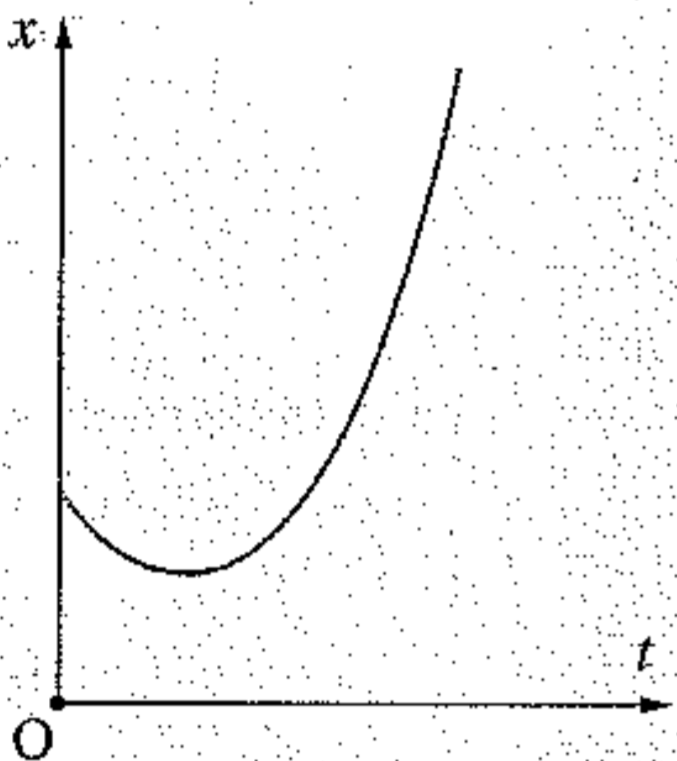
\includegraphics[width=\textwidth]{snelheidsverloop_o}
    \end{image}
    \begin{image}
        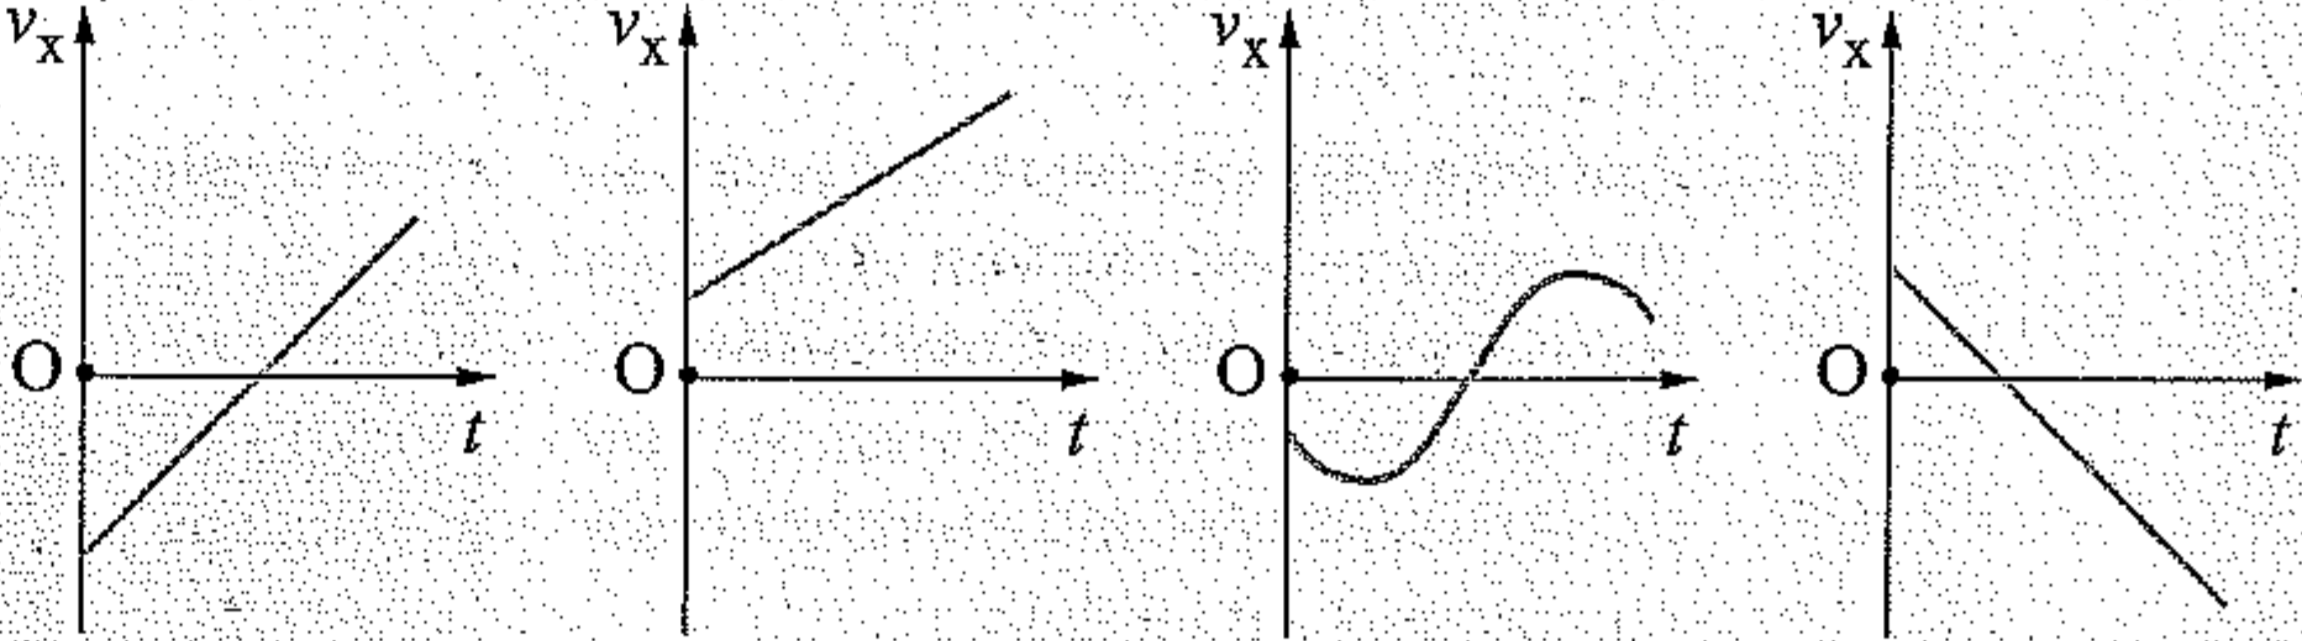
\includegraphics[width=0.93\textwidth]{snelheidsverloop}
    \end{image}
\end{exercise}

\begin{exercise}
Een deeltje beweegt in de zin van de $x$-as. De nevenstaande grafiek geeft aan hoe de grootte van de snelheid verandert als functie van de tijd.
\begin{enumerate}
\item De afstand afgelegd na \SI{15}{s} bedraagt:
\wordChoice{
    \choice{\SI{30}{m}}
    \choice{\SI{120}{m}}
    \choice{\SI{150}{m}}
    \choice{\SI{240}{m}}
}

\item Na \SI{30}{s} heeft het deeltje een welbepaalde afstand afgelegd. Hoe groot zou de constante snelheid van het deeltje moeten zijn om in \SI{30}{s} dezelfde afstand af te leggen?

\wordChoice{
    \choice{\SI{0,0}{m/s}}
    \choice{\SI{6,0}{m/s}}
    \choice{\SI{8,0}{m/s}}
    \choice{\SI{12}{m/s}}
}
\end{enumerate}
\begin{image}
    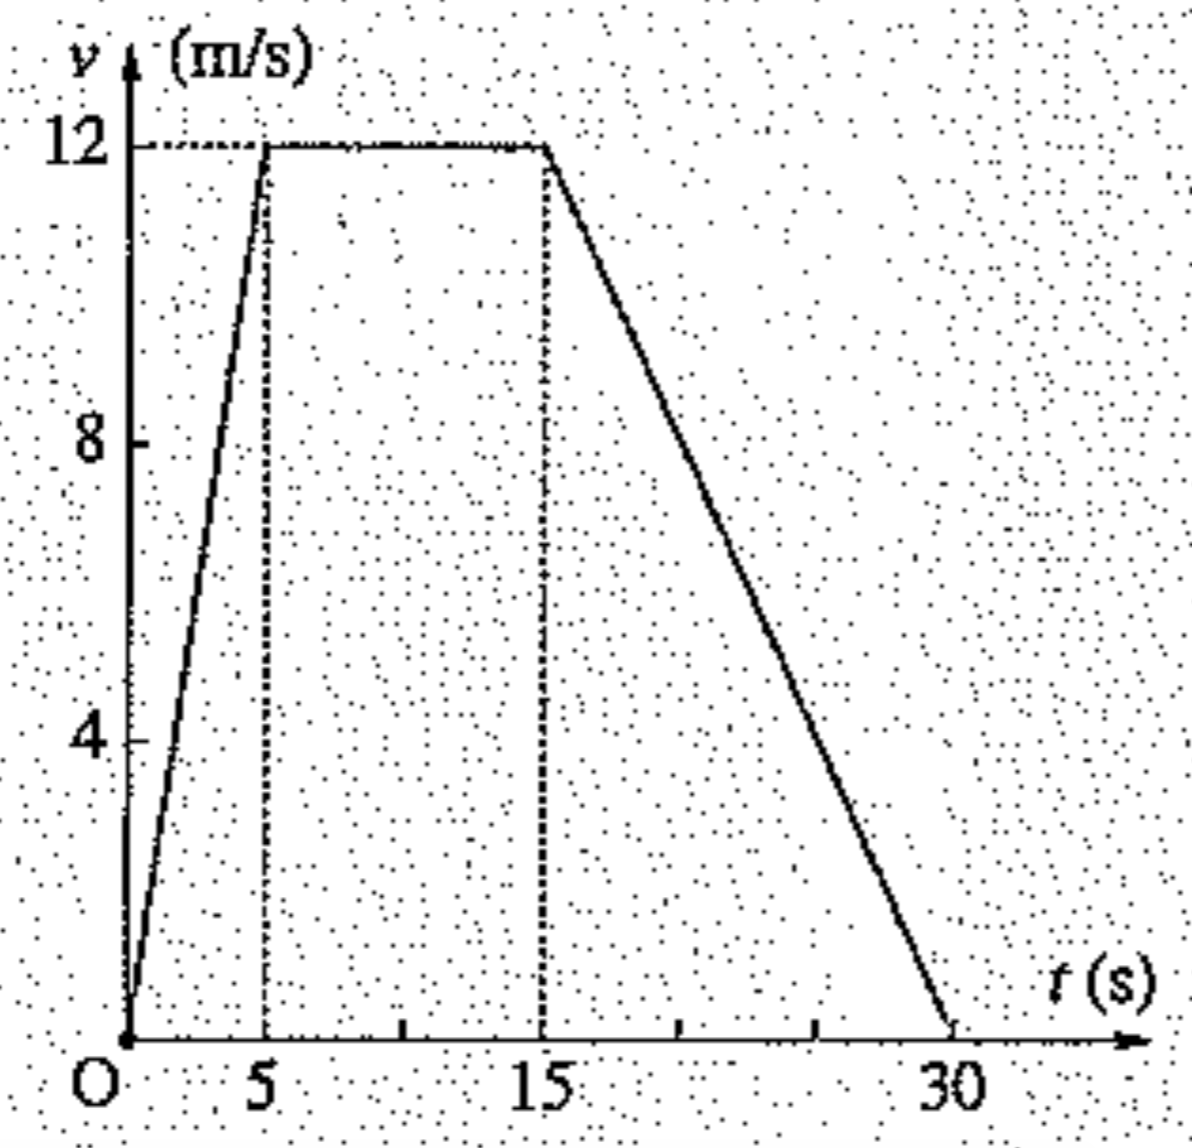
\includegraphics[width=\textwidth]{snelheidsverloop_2_o}
\end{image}
\begin{enumerate}
\setcounter{enumii}{2}
\item Het verloop van de versnellingscomponent van het deeltje wordt kwalitatief voorgesteld op figuur:
\begin{image}
    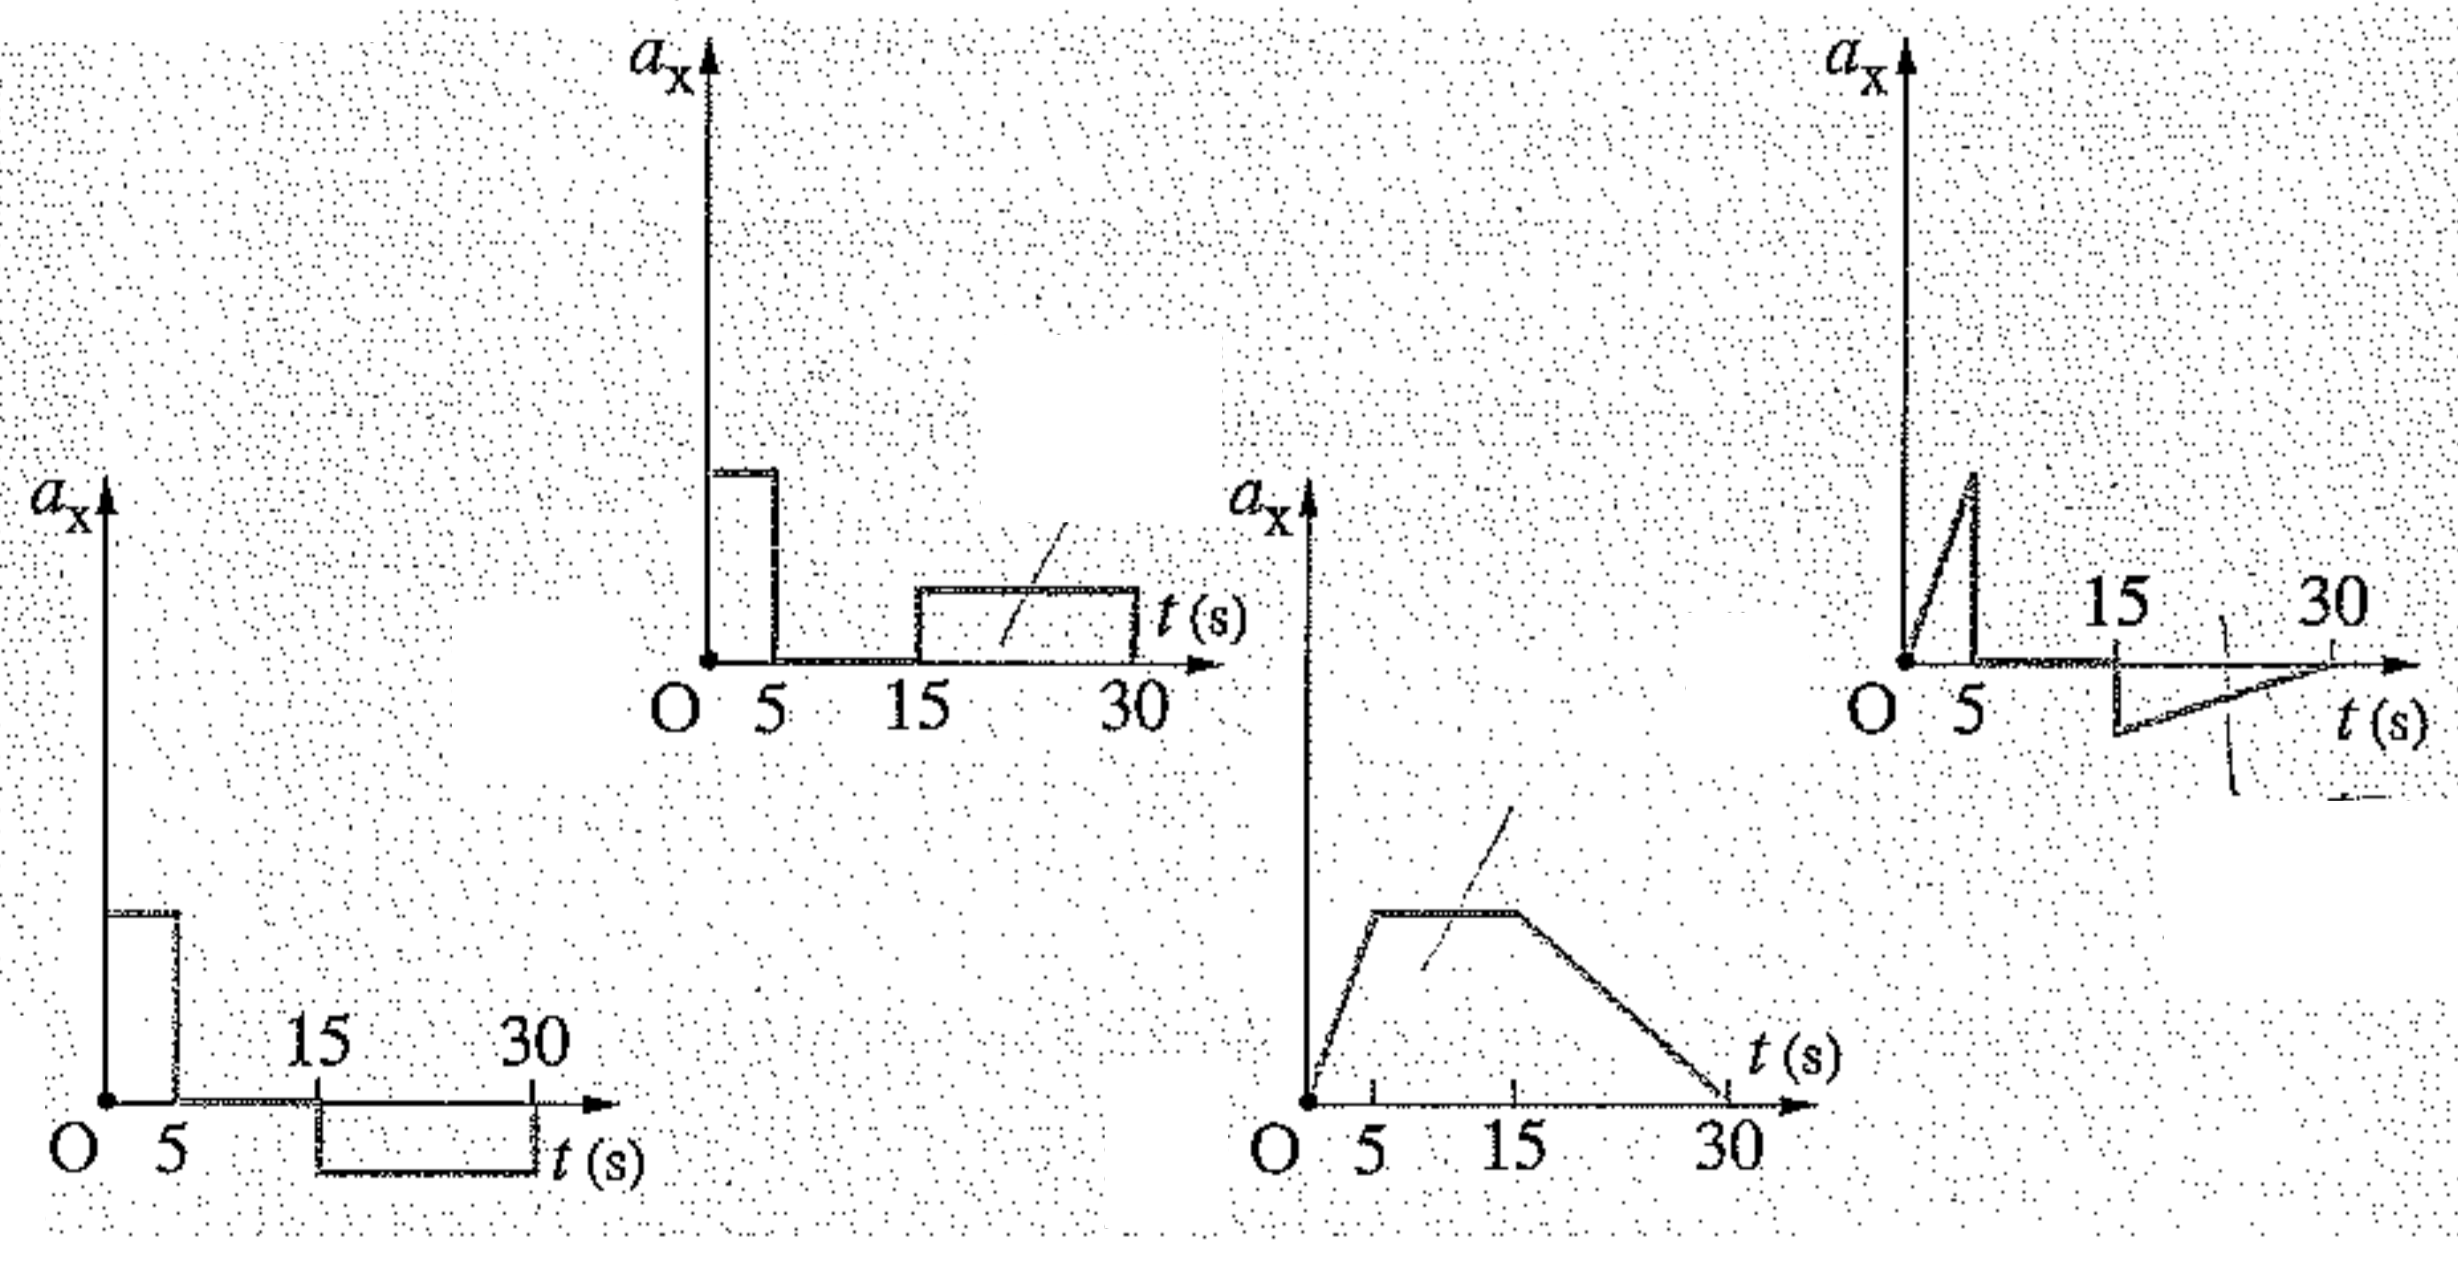
\includegraphics[width=0.93\textwidth]{snelheidsverloop_2}
\end{image}
\end{enumerate}
\end{exercise}

% Bron Serway 4yh edition oefening 77 chapter 2
\begin{exercise}
    (III) Maggie en Jennifer lopen de \SI{100}{m}. Beiden doen ze er exact 10,2 se\-conden over. Met een eenparige versnelling bereikt Maggie na \SI{2}{s} haar maximale snelheid, Jennifer doet dat na \SI{3}{s}. Hun maximale snelheden houden ze aan voor de rest van de wedstrijd.
    \begin{enumerate}
        \item Wat zijn hun maximale snelheden?
        \item Wat is de versnelling van iedere sprinter?
        \item Wie heeft er voorsprong na \SI{6}{s}, en hoeveel?
    \end{enumerate}
    \begin{oplossing}
        $v_1=\frac{2x_2}{2t_2-t_1}$;
        $a=\frac{2x_2}{(2t_2-t_1)t_1}$;
        $x_M-x_J=\frac{2x_2}{2t_2-t_{1,M}}(t-\frac{t_{1,M}}{2})-\frac{2x_2}{2t_2-t_{1,J}}(t-\frac{t_{1,J}}{2})$
        
        Snelheidsgrafiek van Jennifer:
        \begin{image}
            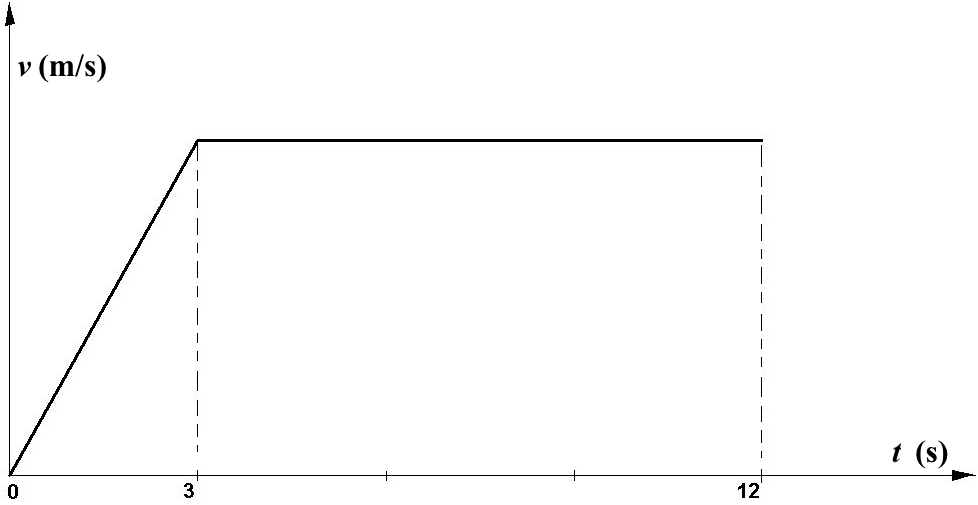
\includegraphics[width=0.5\textwidth]{sprinter}
        \end{image}
    \end{oplossing}
\end{exercise}

\begin{exercise}
    Welke afstand wordt er door een bungeejumper na een vrije val van \SI{2,5}{s} afgelegd?
    \begin{oplossing}
        $x=\frac{1}{2}gt^2=31\rm\,m$
    \end{oplossing}
\end{exercise}

\begin{exercise}
    Een auto die \SI{90}{km/h} rijdt, ligt \SI{100}{m} achter op een vrachtwagen die \SI{75}{km/h} rijdt. Hoeveel tijd kost het de auto om de vrachtwagen in te halen? 
    \begin{oplossing}
        $t=\frac{x_0}{v_a-v_v}=24\rm\,s$
    \end{oplossing}
\end{exercise}

\begin{exercise}
    De snelheid van een trein verandert eenparig in 2 minuten van \SI{20}{km/h} tot \SI{30}{km/h}. De trein rijdt gedurende die tijd over een rechte spoorlijn.
    \begin{enumerate}
        \item Bepaal de versnelling.
        \item Bepaal de afstand die de trein heeft afgelegd gedurende deze 2 minuten.
    \end{enumerate}
\end{exercise}

\begin{exercise}
    Een auto trekt in \SI{5,0}{s} op van \SI{10}{m/s} naar \SI{25}{m/s}. Wat was de versnelling in de veronderstelling dat de auto een EVRB ondergaat? Welke afstand legde de auto in deze periode af?
    \begin{oplossing}
        $a=\frac{v-v_0}{t-t_0}=3\rm\,m/s$,
        $x-x_0=\left(\frac{v_0+v}{2}\right)(t-t_0)=87,5\rm\,m$
    \end{oplossing}
\end{exercise}

\begin{exercise}
    Bij het katapulteren van vliegtuigen wordt een startbaan van \SI{25,0}{m} gebruikt, die door het vliegtuig eenparig versneld in \SI{1,00}{s} wordt doorlopen. Zoek zijn versnelling en de snelheid waarmee het de baan verlaat.
\end{exercise}

\begin{exercise}
    Een auto trekt op tot \SI{100}{km/h} in \SI{6,0}{s}. Als hij dat doet op een rechte baan met constante versnelling, welke afstand is er dan hiervoor nodig?
    \begin{oplossing}
        $a=\frac{v}{t}=4,63\rm\,m/s^2$, $x=\frac{vt}{2}=83,3\rm\,m$
    \end{oplossing}
\end{exercise}

\begin{exercise}
    Een auto vertrekt vanuit rust en bereikt na \SI{3,0}{km} een snelheid van \SI{450}{km/h} We onderstellen de versnelling constant en de baan recht. Bereken de versnelling en de tijd, nodig om die \SI{3,0}{km} af te leggen.
    \begin{oplossing}
    % \footnote{$t=\frac{2x}{v}=48\rm\,s$, $a=\frac{v^2}{2x}=2,6\rm\,m/s^2$}
    % \item[gegeven]$x=3000\rm\,m$\newline $v=125\rm\,m/s$
    % \item[gevraagd]$a$, $t$
    % \item[oplossing]
    Omdat voor een EVRB de gemiddelde snelheid gegeven wordt door $\overline{v}=\frac{v_0+v}{2}$ en we de afgelegde afstand kennen, kunnen we de benodigde tijd gemakkelijk vinden. We kiezen $t_0=0$, $x_0=0$. De beginsnelheid is nul zodat:
    \begin{eqnarray*}
    \Delta x &=& \overline{v}\Delta t \\
    &\Downarrow & \\
    t &=& \frac{x}{\left(\frac{v}{2}\right)} = \frac{2x}{v}
    \end{eqnarray*}
    Invullen van de gegevens levert een tijd van \SI{48}{s}. Met het formuletje voor de snelheid vinden we de versnelling door de tijd te substitueren:
    \begin{eqnarray*}
    v &=& at \\
    &\Updownarrow&\\
    a &=& \frac{v}{t}=\frac{v}{\left(\frac{2x}{v}\right)}\\
    &=& \frac{v^2}{2x}
    \end{eqnarray*}
    Invullen van de gegeven grootheden levert een versnelling van \SI{2,6}{m/s^2}.
    \end{oplossing}
\end{exercise}

\begin{exercise}
    Een vliegtuig landt met een snelheid van \SI{100}{m/s}. Op de ladingsbaan heeft het een vertraging van \SI{5,0}{m/s^2}. Welke afstand heeft het vliegtuig nodig om tot stilstand te komen?
\end{exercise}

\begin{exercise}
    Een trein vertrekt uit een station en rijdt met een eenparig versnelde beweging waarvan de versnelling \SI{0,50}{m/s^2} bedraagt. Hoe groot is de afstand die de trein heeft afgelegd als zijn snelheid \SI{72,0}{km/h} bedraagt?
\end{exercise}

\begin{exercise}
    Twee personen A en B voeren op dezelfde rechte en vanuit dezelfde beginstand een eenparige beweging uit. A vertrekt \SI{100}{s} eerder dan B. Met een snelheid die dubbel zo groot is als die van A haalt B, op \SI{400}{m} van het vertrekpunt, A in. Bereken beide snelheden en stel ze grafisch voor.
    %\begin{oplossing}
    %\item[gegeven]$x_0=1,00\cdot10^3\rm\,m$\newline$t_0=100\rm\,s$\newline$v_b=-2v_a$\newline$x=400\rm\,m$
    %\item[gevraagd]$v_a$, $v_b$
    %\item[oplossing]De bewegingsvergelijkingen voor A en B worden gegeven door:
    %\begin{eqnarray}
    %A:\qquad x&=&v_at \label{verg A}\\
    %B:\qquad x&=&x_0+v_b(t-t_0)\nonumber\\
    %&=&x_0-2v_a(t-t_0) \label{verg B}
    %\end{eqnarray}
    %De grafiek van beide functies ziet er als volgt uit:
    %\begin{image}}[h]
    %\centering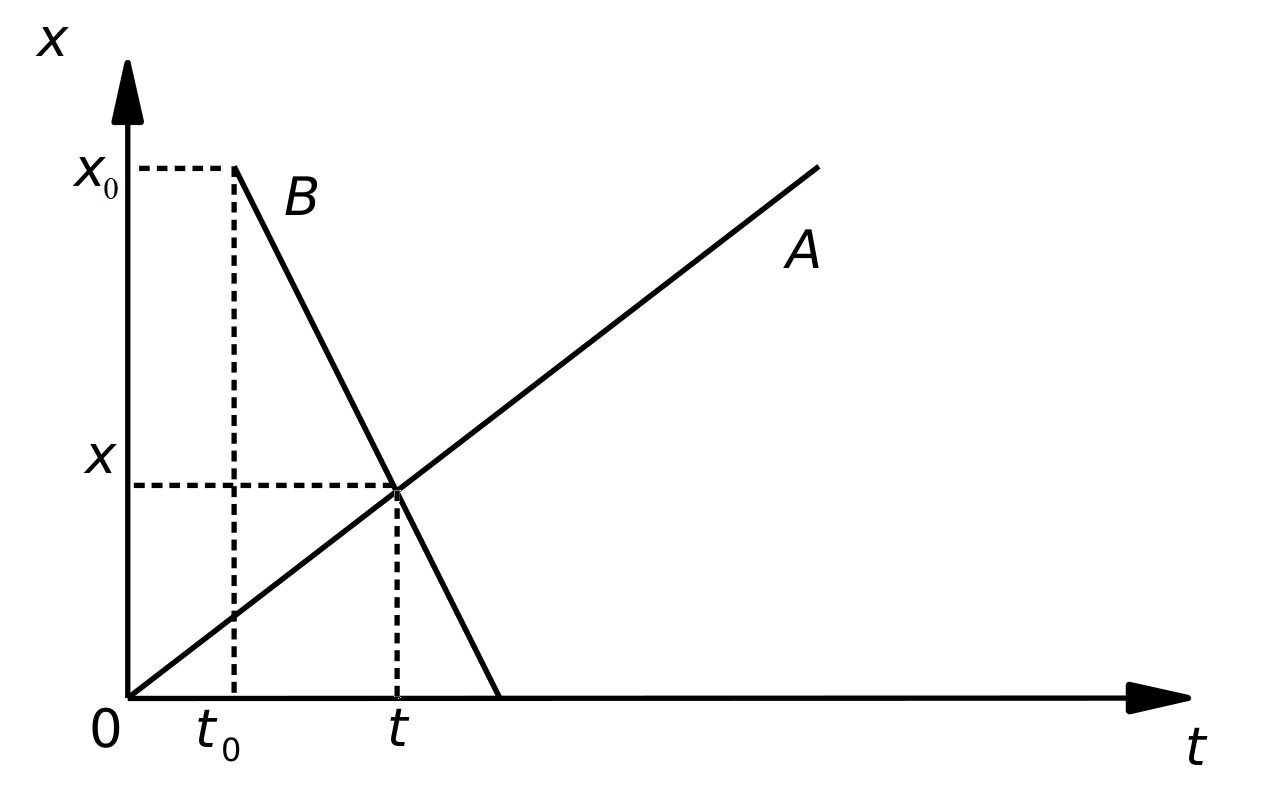
\includegraphics[width=0.6\textwidth]{38p40}
    %\end{image}}
    %\newline
    %Als we voor $x$ de ontmoetingsplaats van \SI{400}{m} nemen, hebben we twee vergelijkingen (\ref{verg A}), (\ref{verg B}) en twee onbekenden $t$, $v_a$. Dit kunnen we oplossen door een variabele te substitueren. We nemen de tijd, $(\ref{verg A})\Leftrightarrow t=\frac{x}{v_a}$ en substitueren deze in vergelijking (\ref{verg B}):
    %\begin{eqnarray*}
    %x&=&x_0-2v_a(t-t_0)\\
    %&=&x_0-2v_a\left(\frac{x}{v_a}-t_0\right)\\
    %&\Updownarrow&\\
    %v_a&=&\frac{3x-x_0}{2t_0}=1,0\rm\,m/s
    %\end{eqnarray*}
    %En de snelheid van B:
    %\begin{equation}
    % v_b=-2v_a=\frac{x_0-3x}{t_0}=-2,0\rm\,m/s
    %\end{equation} 
    %\end{oplossing}
\end{exercise}

\begin{exercise}
    Een vliegtuig start vanuit rust en versnelt met een constante versnelling langs de grond alvorens op te stijgen. Het legt \SI{600}{m} af in \SI{12}{s}. Bepaal de versnelling, de snelheid na \SI{12}{s} en de afstand afgelegd gedurende de twaalfde seconde.

    \begin{oplossing}
        $a=\frac{2x}{t^2}=\SI{8,33}{m/s^2}$,
        $v=\frac{2x}{t}=\SI{100}{m/s}$,
        $x(t=12)-x(t=11)=\frac{1}{2}a(t_{12}^2-t_{11}^2)=\SI{95,8}{m}$
    \end{oplossing}
\end{exercise}


\end{document}
